\subsection{Objective and binarising the data set}
This section presents the results of performing association mining on the glass data using the Apriori algorithm \cite[Section 19, algorithm 8]{coursenotes}.

The association mining is done on a binarized version of our data set where each observation is not described by continuous attributes, but instead as having either a low value of the attribute (below or equal to the 50th percentile) or a high value (above the 50th percentile). This means that each of the 9 continuous attributes, e.g. \texttt{RI}, is transformed into 2 new binary attributes called $\low{RI}$ and $\high{RI}$. The \texttt{type} attribute has also been binarized by 1-out-of-K coding, i.e. transformed into 7 binary attributes called \texttt{building float}, \texttt{building non-float}, (...), and \texttt{headlamps}. Thus, the binarized data set consists of $9\cdot2 + 7 = 25$ binary attributes, or \textit{items} as they are customarily called in the context of association mining.

The objective can now be expressed more concretely as finding frequent item sets and association rules with high confidence from this data set. %kan uddybes

\subsection{Frequent itemsets}


\begin{figure}[H]
    \centering
    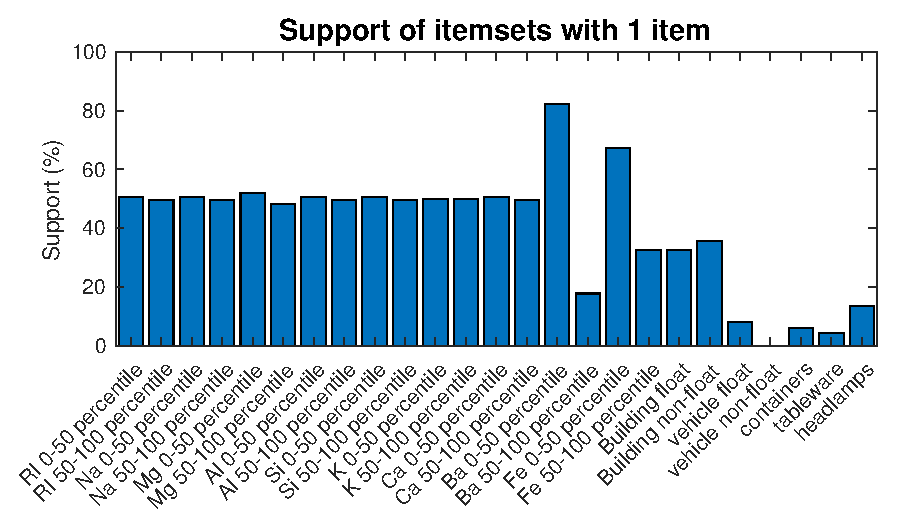
\includegraphics[width = 0.7\textwidth]{fig/freq-items-plot.eps}
    \caption{Plot of the support of each of the 25 items in the binarized data set.}
    \label{fig:freq-items-plot}
\end{figure}

Figure 1 shows a plot the frequency of each of the 25 items in the binarized data set. The plot shows that while most of the items corresponding to the continuous attributes have frequencies around 50\% as should be expected, \texttt{Ba} and \texttt{Fe} sticks out with respectively 82\% and 67\% of their values being low values (in the 0-50 percentile range). This is imbalance is explained by the fact that 82\% of the \texttt{Ba} values and 67\% of the \text{Fe} values are 0. Furthermore, the \texttt{type} items (\texttt{building float}, \texttt{building non-float}, etc.) all have significantly lower frequencies than the continuous attributes. This is of course explained by the fact that \texttt{type} have been split into 7 items (6 if we ignore the empty class \texttt{vehicle non-float}) rather than 2 items for the other attributes.

\begin{table}[H]
    \centering
    \begin{tabular}{l|l|l}
        top 5 sets of 1 item  & top 5 sets of 2 items   & top 5 sets of 3 items \\ \hline
        %     $\texttt{Ba}_{(0\%-50\%)}$ (82\%) 
        % &   $\{\texttt{Ba}_{(0\%-50\%)}$, $\texttt{Fe}_{(0\%-50\%)}$\} (56\%)
        % &   $\{\texttt{K}_{(50\%-100\%)}$, $\texttt{Na}_{(0\%-50\%)}$, $\texttt{Ba}_{(0\%-50\%)}$\} (35\%)\\
        %     $\texttt{Ba}_{(0-50)}$ (82\%) 
        % &   $\{\texttt{Ba}_{(0-50)}$, $\texttt{Fe}_{(0-50)}$\} (56\%)
        % &   $\{\texttt{K}_{(50-100)}$, $\texttt{Na}_{(0-50)}$, $\texttt{Ba}_{(0-50)}$\} (35\%)\\  
            $\{\low{Ba}\}$ (82\%) 
        &   \{$\low{Fe}$, $\low{Ba}$\} (56\%)
        &   $\{ \high{K}$, $\low{Na}$, $\low{Ba}\}$ (35\%)\\  
        % ny række
            $\{\low{Fe}\}$ (67\%) 
        &   $\{\low{Al}$, $\low{Ba}$\} (48\%) 
        &   $\{\low{RI}$, $\low{Ca}$, $\low{Ba}\}$ (34\%)\\
        % ny række
            $\{\low{Mg}\}$ (52\%)
        &   $\{\low{Na}$, $\low{Ba}\}$ (47\%) 
        &   $\{ \high{RI}$, $\high{Ca}$, $\low{Ba}\}$ (34\%)\\
        % ny række
            $\{\low{Ca}\}$ (50\%) 
        &   $\{\low{Si}$, $\low{Ba}$\} (46\%) 
        &   $\{ \high{RI}$, $\low{Si}$, $\low{Ba}\}$  (33\%)  \\
        % ny række
            $\{\low{Al}\}$ (50\%) 
        &   $\{\high{Mg}$, $\low{Ba}\}$ (46\%) 
        &   $\{ \low{Al}$, $\low{Fe}$, $\low{Ba}\}$ (32\%) \\
    \end{tabular}
    \caption{Table of the top 5 most frequent item sets consisting of either 1, 2, or 3 items. The bracketed percentages are the supports of the item sets.}
    \label{tab:freq-items}
\end{table}

The effects of these imbalances are seen in Table \ref{tab:freq-items}, that displays the top 5 most frequent itemsets of size 1, 2, and 3, found by the Apriori algorithm. We observe that

\begin{itemize}
    \item The most frequent set of 2 items is $\{\low{Fe},\low{Ba} \}$, containing the two most frequent items.
    \item All of the sets of 2 and 3 items include the most frequent item $\low{Ba}$.
    \item None of the item sets in the table include any \texttt{type} items.
\end{itemize}

In other words, most of the most frequent item sets are uninteresting, as they tell us very little about our data. However, if we ignore the $\low{Ba}$ item, the top 5 sets of 3 items do carry some interesting results: $\{ \low{RI}$,$\low{Ca} \}$ as well as $ \{ \high{RI}$,$\high{Ca} \}$ are frequently occurring pairs which match up with the strong correlation of 0.81 between \texttt{Ca} and \texttt{RI}, as found in report 1. Similarly, the high frequency of  \{$\high{RI},\low{Si}$\} is explained by a fairly high negative correlation between \texttt{RI} and \texttt{Si} of $-0.54$. But at the top of the list is \{$\high{K},\low{Na}$\} despite a weaker correlation of $-0.27$ and none of the items occurring in the top 5 most frequent single items. In other words, this item set is non-trivially frequent and arguably the juiciest fruit of this part of the analysis.

\subsection{Association rules}

\begin{table}[H]
\centering
\begin{tabular}{c c l c c}
    No. & Rule  & & Support & Confidence  \\ \hline
    % ny række
    1   &$\{\high{Mg}$, $\low{Ca}$, $\low{Fe} \}$ &$\rightarrow\{\low{Ba}\}$ 
    & 21.5\% & 100\% \\
    % ny række
    2   &$\{\low{Ca}$, $\low{Na}$, $\low{Fe} \}$ &$\rightarrow\{\low{Ba}\}$ 
    & 20.1\% & 100\% \\
    % ny række
    3   &$\{\low{RI}$, $\low{Na}$, $\low{Fe} \}$ &$\rightarrow\{\low{Ba}\}$ 
    & 19.6\% & 100\% \\
    % ny række
    4   &$\{\high{Mg}$, $\high{K}$, $\low{Fe} \}$ &$\rightarrow\{\low{Ba}\}$ 
    & 19.2\% & 100\% \\
    % ny række
    5   &$\{ \high{Al}, \high{Ca} \}$  &$\rightarrow \{ \low{Mg} \} $
    & 19.1\% & 100\% \\
    % ny række
    6   &$\{\high{Mg}$, $\low{RI}$, $\low{Fe} \}$ &$\rightarrow\{\low{Ba}\}$ 
    & 18.2\% & 100\% \\ 
    % ny række
    7   &$\{ \texttt{Building float}, \high{Ca} \}$ &$\rightarrow \{ \low{Al} \} $
    & 17.3\% & 100\% \\
    % ny række
    8   &$\{\high{Mg}$, $\low{Na}$, $\low{Fe} \}$ &$\rightarrow\{\low{Ba}\}$ 
    & 16.4\% & 100\% \\
    % ny række
    9   &$\{\texttt{Building non-float}$, $\low{Ca}$, $\low{Fe} \}$ &$\rightarrow\{\low{Ba}\}$ 
    & 16.4\% & 100\% \\
    % ny række
    10  &$\{\texttt{Building float}, \high{Ca}, \low{Ba} \}$ &$\rightarrow \{\low{Al}\}$
    & 16.4\% & 100\% \\
    % ny række 
    11  &$\{ \low{RI}, \low{Al} \}$ &$\rightarrow \{ \low{Ba} \} $
    & 16.4\% & 100\% \\
    %ny række
    12  &$\{ \high{Mg}, \high{Ca} \}$ &$\rightarrow \{ \low{Al} \} $
    & 16.4\% & 100\% \\
\end{tabular}
\caption{The 12 association rules of confidence = 100\% with the highest support.}
\label{tab:assoc-rules}
\end{table}
Since the binarized data set is 25-dimensional, a huge number of association rules may be extracted from it. The way we have chosen to constrain our search is to only look for association rules with 100\% confidence. Of course, the trade-off of high confidence is low support, but in some sense, this is an advantage since it allows the \texttt{type} items to play a role. Other approaches are also valid, but we found this one to generate the most interesting results.

In Table \ref{tab:assoc-rules} is seen the top 12 association rules with 100\% confidence sorted by support. From this we observe the following points:

\begin{itemize}
    \item $\low{Ba}$ is the implication of most of the association rules. These rules are unsurprising and mainly uninteresting for the reasons laid out in the former subsection. Also, $\low{Fe}$ is present in many of the rules which may also be explained by the high frequency of this item rather than a meaningful association.
    \item Most of the found association rules $X \rightarrow Y$ have that $|X|$ (the number of items in $X$) is 3. the other rules have $|X|=2$, while none of them have $|X|= 1$. This is also expected, since one would require knowledge about a lot of items to deduce something with a lot of confidence.
    \item 3 of the 12 rules include a \texttt{type} item. For instance, we see that from rule No. 7 that a low percentage of \texttt{Al} is implied by a high percentage of $\texttt{Ca}$ and the glass being of type \texttt{Building float}. Only the two most frequent \texttt{type}s are included, which is not surprising; Finding association rules that involve the other types will naturally have even lower support. Also, none of the association rules listed here imply any \texttt{type}s, and can thus not be used for classification.
\end{itemize}

While one could walk through each of these association rules and try to interpret them or explain them from the data, it must be stressed that they should be cross-validated on a new data set, on which they may well not have confidence of 100\%. Since these rules are not checked with cross-validation, one should not be too quick to derive information on the properties of glass from them.  The reason that cross-validation has not been used in this analysis is mainly because of technical limitations in the way the Apriori algorithm is implemented in our machine learning toolbox.